% 第三章建議使用 16 張方法圖，依各段位置分別插入。
% 每段均包含前導文字、圖說、標籤與圖檔路徑。
% 門與抽屜改成獨立圖，取代原 articulated_operation_constraints 合併圖。
% 原合併圖僅保留為備用，不與獨立圖重複插入。
% PDF 已嵌入標楷體；圖片為方法說明，非實驗結果。

% 本檔僅列本次新增與拆分的 11 張圖片。

% ==================================================
% 3.1.2 底盤參考位姿、實際位姿與相對幾何關係
% 位置：3.1.2 幾何追蹤誤差與局部模型說明之後
% ==================================================
底盤位姿的相對幾何關係如\cref{fig:ch3_base_pose_error}所示。圖中 $t_E=R_r^{\top}(p_B-p_r)$ 為相對變換的平移分量；幾何誤差 $e_B$ 則由完整相對位姿的對數映射取得，兩者依各自定義使用。

\begin{figure}[htbp]
    \centering
    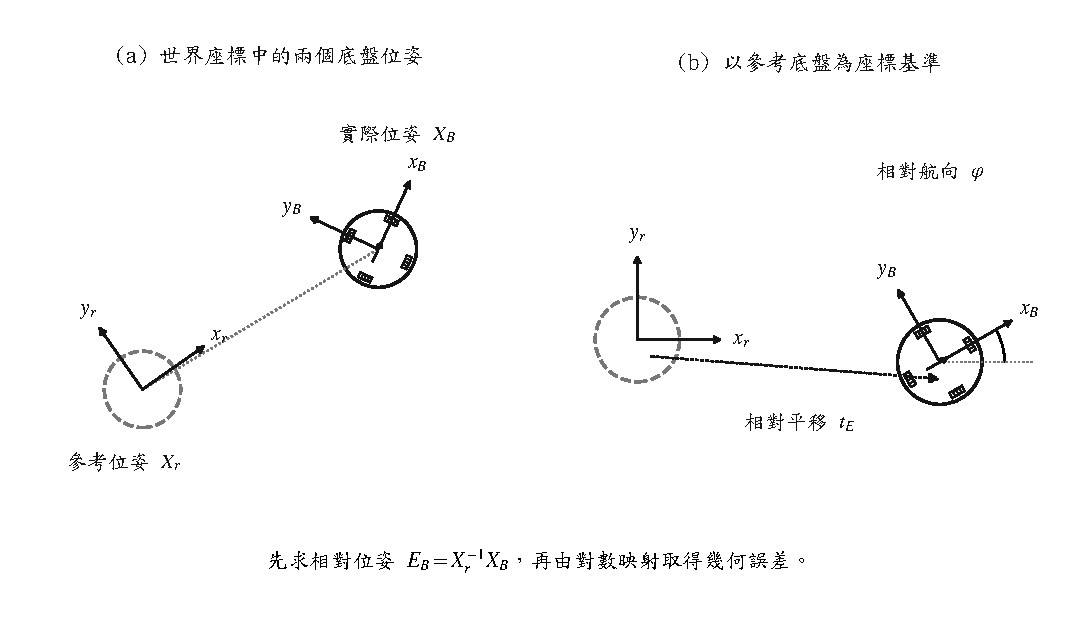
\includegraphics[width=0.98\textwidth]{figsrc/ch03/base_pose_error.pdf}
    \caption{底盤參考位姿、實際位姿與相對幾何關係}
    \label{fig:ch3_base_pose_error}
\end{figure}


% ==================================================
% 3.1.3 底盤側移時之手臂構型調整與末端位置保持
% 位置：3.1.3 正向運動學公式及其說明之後
% ==================================================
底盤與手臂的運動學耦合如\cref{fig:ch3_wholebody_motion_coupling}所示。兩個構型對應相同的世界座標末端目標；底盤側移時，手臂配合調整關節構型，使末端保持在操作目標附近。

\begin{figure}[htbp]
    \centering
    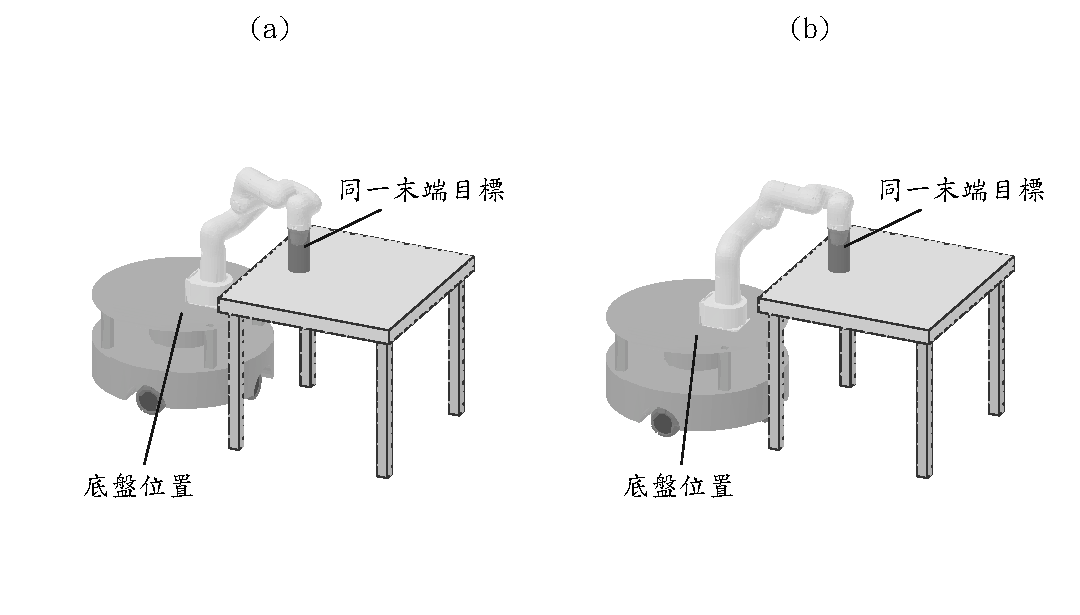
\includegraphics[width=0.98\textwidth]{figsrc/ch03/wholebody_motion_coupling.pdf}
    \caption{底盤側移時之手臂構型調整與末端位置保持}
    \label{fig:ch3_wholebody_motion_coupling}
\end{figure}


% ==================================================
% 3.3.3 底盤與手臂於同一全身控制問題中共同求解
% 位置：3.3.3 最佳化問題及數值求解說明之後
% ==================================================
共同求解的輸入與輸出關係如\cref{fig:ch3_joint_optimization}所示。導航參考與末端操作目標共同作用於同一控制序列，配合增廣模型及限制條件，同時決定底盤速度命令與手臂設定點變化率。

\begin{figure}[htbp]
    \centering
    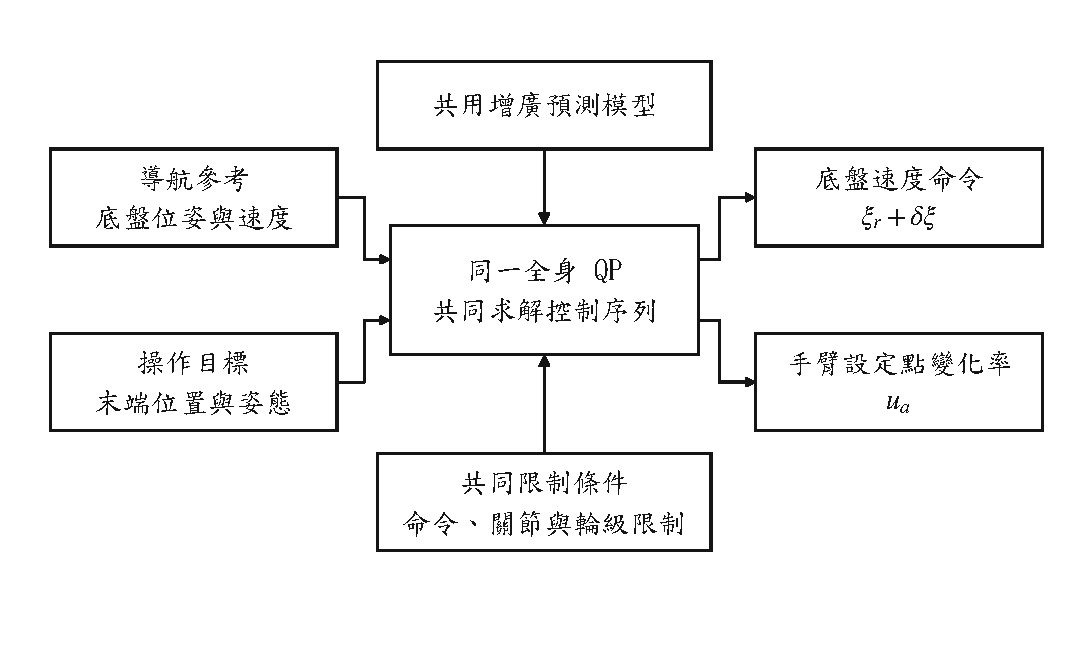
\includegraphics[width=0.98\textwidth]{figsrc/ch03/joint_optimization.pdf}
    \caption{底盤與手臂於同一全身控制問題中共同求解}
    \label{fig:ch3_joint_optimization}
\end{figure}


% ==================================================
% 3.4.5 導航參考調整、預測避障與底盤命令處理之分層關係
% 位置：3.4.5 原始掃描防護與命令處理說明之後
% ==================================================
各層的作用位置如\cref{fig:ch3_navigation_command_layers}所示。參考調整改變導航目標序列，CBF 作用於全身最佳化問題，雷射防護與輪級限制則依序處理待執行底盤命令；最終放行值回報後，供後續命令限制與運動預測使用。

\begin{figure}[htbp]
    \centering
    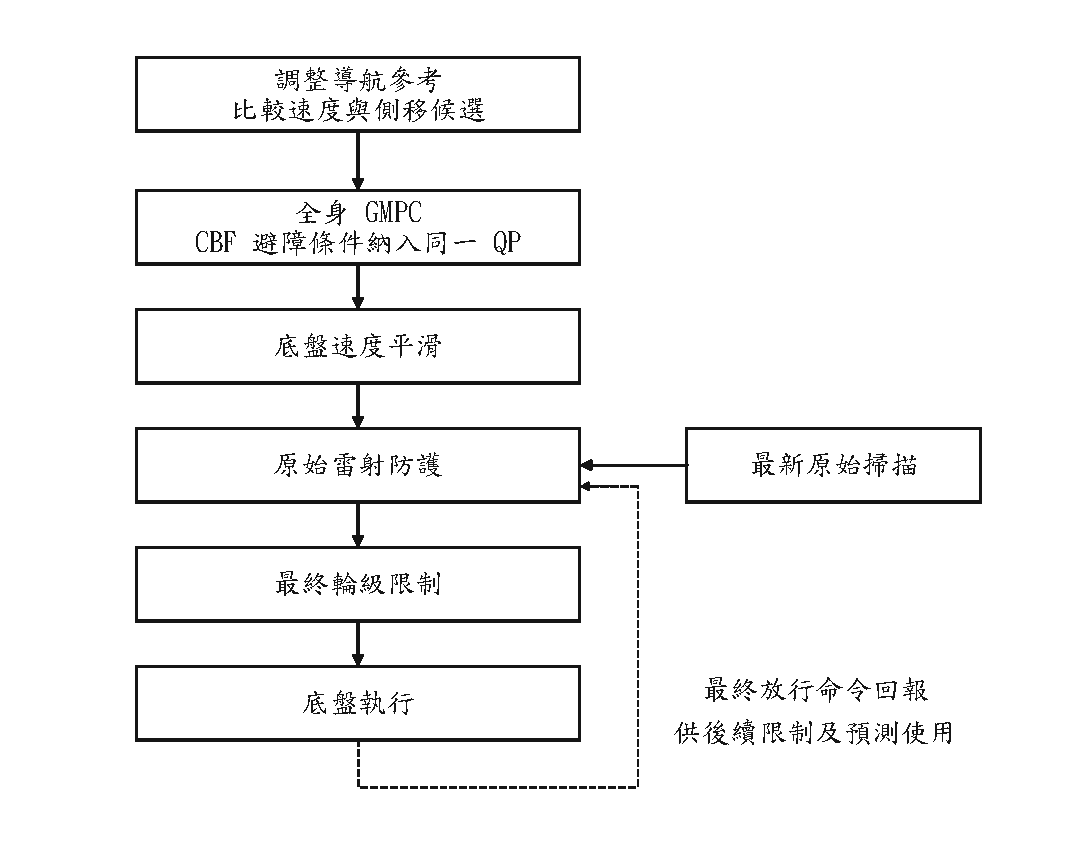
\includegraphics[width=0.98\textwidth]{figsrc/ch03/navigation_command_layers.pdf}
    \caption{導航參考調整、預測避障與底盤命令處理之分層關係}
    \label{fig:ch3_navigation_command_layers}
\end{figure}


% ==================================================
% 3.5.2 視覺量測與相機位姿依觀測時間配對之流程
% 位置：3.5.2 影像時間對齊說明之後
% ==================================================
視覺量測與相機位姿的時間配對如\cref{fig:ch3_visual_time_alignment}所示。影像處理完成後仍保留原觀測時間 $t_o$，並使用該時刻的相機位姿進行座標轉換，再將世界座標中的目標提供給操作參考生成。

\begin{figure}[htbp]
    \centering
    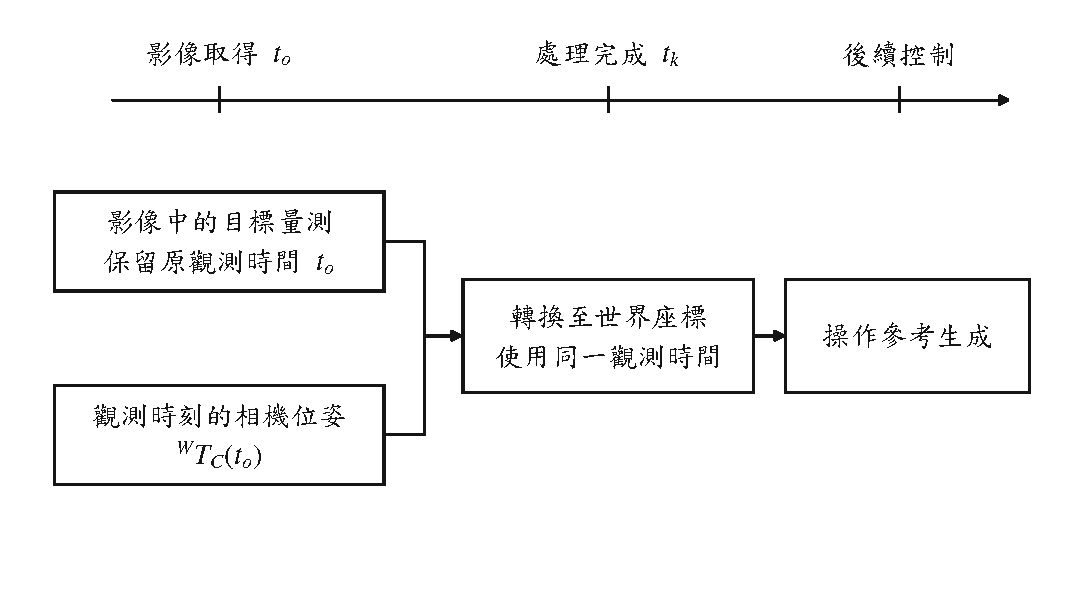
\includegraphics[width=0.98\textwidth]{figsrc/ch03/visual_time_alignment.pdf}
    \caption{視覺量測與相機位姿依觀測時間配對之流程}
    \label{fig:ch3_visual_time_alignment}
\end{figure}


% ==================================================
% 3.6.1 接近、閉爪確認與抓持成立之狀態轉移
% 位置：3.6.1 抓持證據與連接確認說明之後
% ==================================================
抓持狀態的轉移如\cref{fig:ch3_grasp_state_transition}所示。閉爪命令發出後，需檢查手指位置與接觸證據，待條件持續成立並取得必要的連接確認後，才銜接抓持後的機構操作或持物運送。

\begin{figure}[htbp]
    \centering
    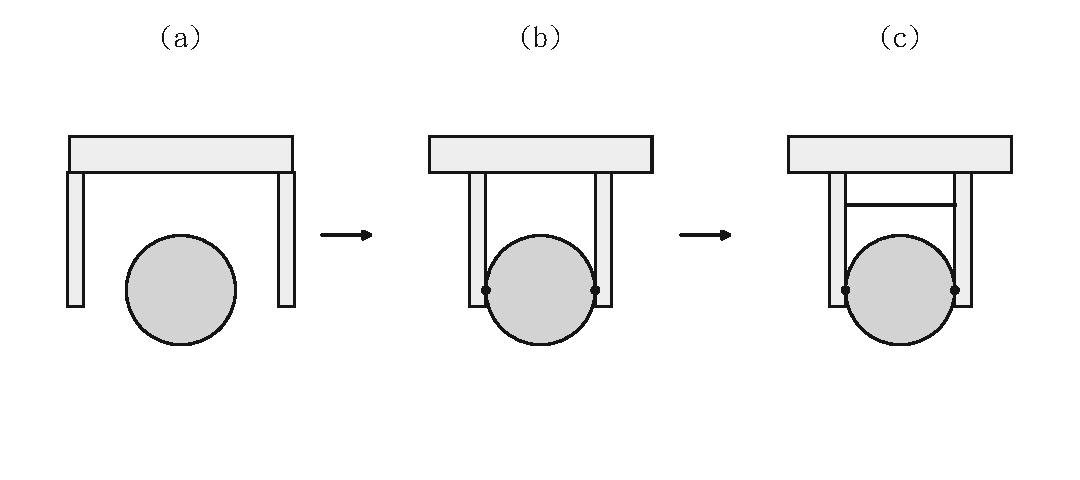
\includegraphics[width=0.98\textwidth]{figsrc/ch03/grasp_state_transition.pdf}
    \caption{接近、閉爪確認與抓持成立之狀態轉移}
    \label{fig:ch3_grasp_state_transition}
\end{figure}


% ==================================================
% 3.6.2 開門前後之門扇、底盤與手臂構型
% 位置：3.6.2 旋轉門模型與門角更新說明之後
% ==================================================
不同門角下的協同構型如\cref{fig:ch3_door_operation_sequence}所示。把手繞鉸鏈運動時，底盤位置與手臂構型配合調整，並維持式\eqref{eq:ch3_grasp_closed_chain}所定義的抓持相對位姿。

\begin{figure}[htbp]
    \centering
    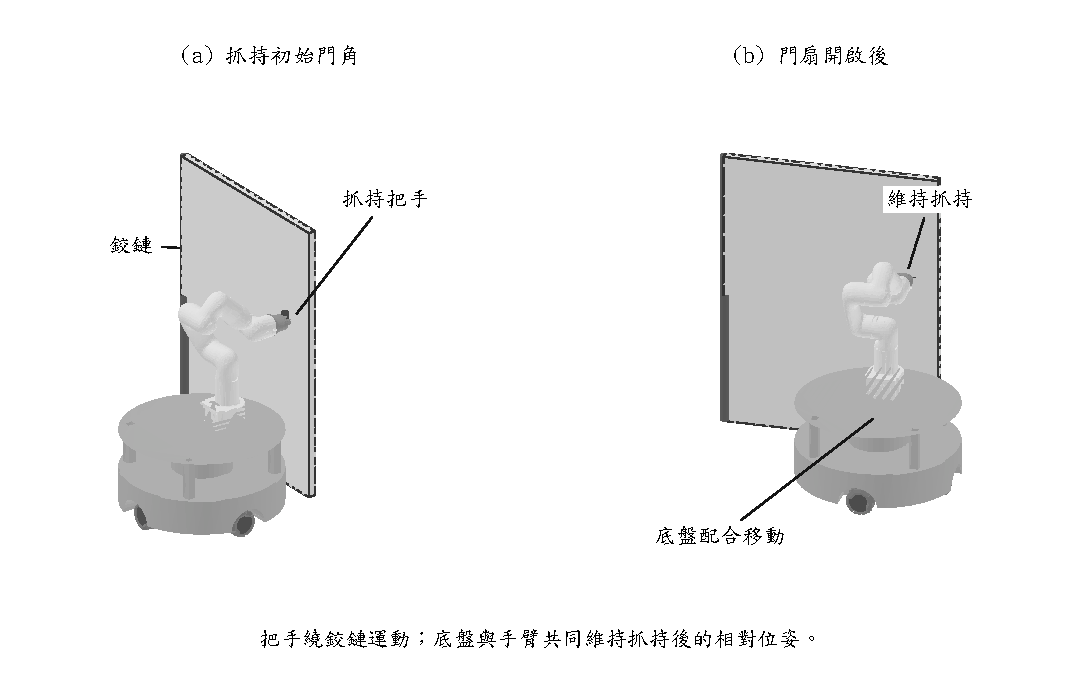
\includegraphics[width=0.98\textwidth]{figsrc/ch03/door_operation_sequence.pdf}
    \caption{開門前後之門扇、底盤與手臂構型}
    \label{fig:ch3_door_operation_sequence}
\end{figure}


% ==================================================
% 3.6.2 抽屜拉出前後之滑軌位移與全身構型
% 位置：3.6.2 平移抽屜模型與有效行程說明之後
% ==================================================
抽屜拉出前後的機構位移與全身構型如\cref{fig:ch3_drawer_operation_sequence}所示。抽屜沿滑軌平移並保持機構姿態，底盤與手臂則依操作進度更新參考，以維持抓持及所需的運動空間。

\begin{figure}[htbp]
    \centering
    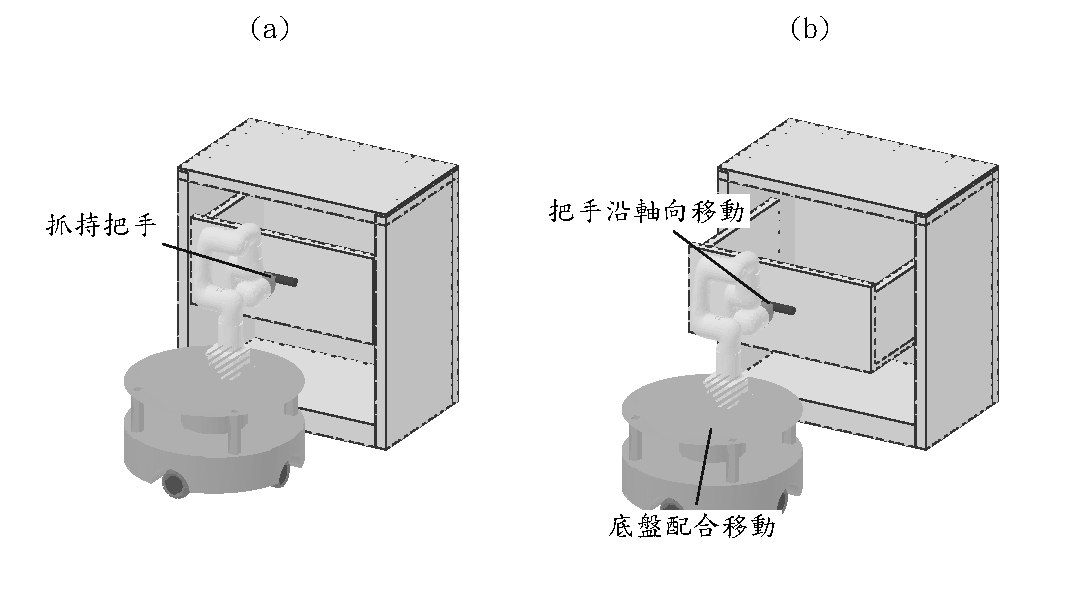
\includegraphics[width=0.98\textwidth]{figsrc/ch03/drawer_operation_sequence.pdf}
    \caption{抽屜拉出前後之滑軌位移與全身構型}
    \label{fig:ch3_drawer_operation_sequence}
\end{figure}


% ==================================================
% 3.6.3 相對底盤目標下之持物運送與構型保持
% 位置：3.6.3 持物相對目標與運送流程說明之後
% ==================================================
相對底盤目標下的運送關係如\cref{fig:ch3_base_relative_carrying}所示。手臂維持相對底盤的末端構型時，物件在世界座標中的位置隨底盤一起改變。此關係由式\eqref{eq:ch3_base_relative_carry_target}建立，與前述世界固定操作目標分別處理。

\begin{figure}[htbp]
    \centering
    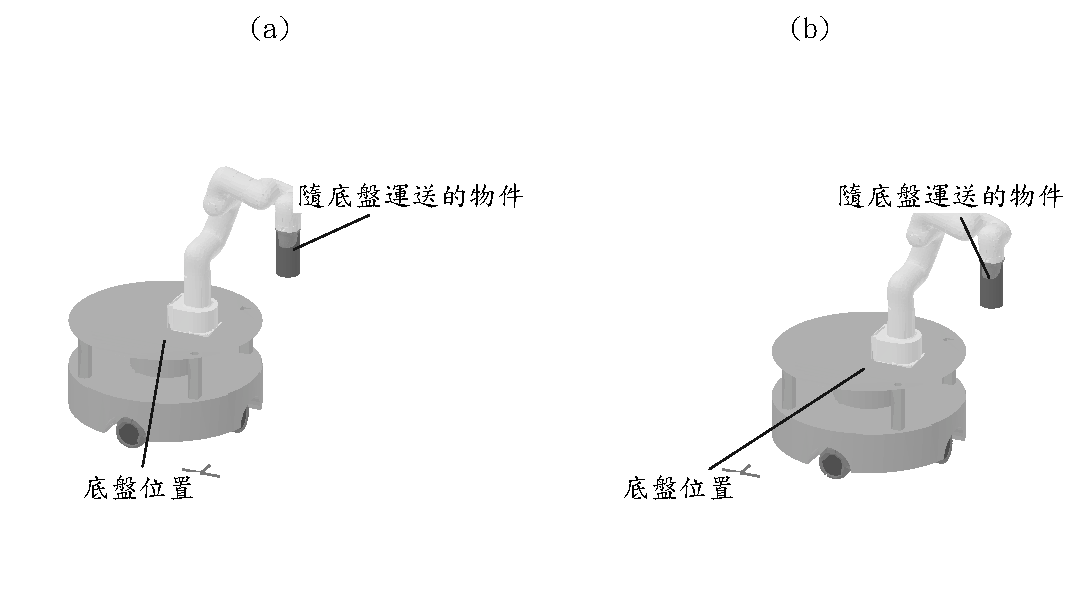
\includegraphics[width=0.98\textwidth]{figsrc/ch03/base_relative_carrying.pdf}
    \caption{相對底盤目標下之持物運送與構型保持}
    \label{fig:ch3_base_relative_carrying}
\end{figure}


% ==================================================
% 3.7.2 模型偏置估測之區間殘差與共用模型更新
% 位置：3.7.2 模型偏置估測說明之後、TCP 補償介紹之前
% ==================================================
模型偏置估測的更新位置如\cref{fig:ch3_model_bias_estimation}所示。區間末殘差先由更新前的偏置估計計算，經平滑與限幅後，再將新偏置提供給後續 QP 預測、在途命令前推與停止軌跡核對使用。

\begin{figure}[htbp]
    \centering
    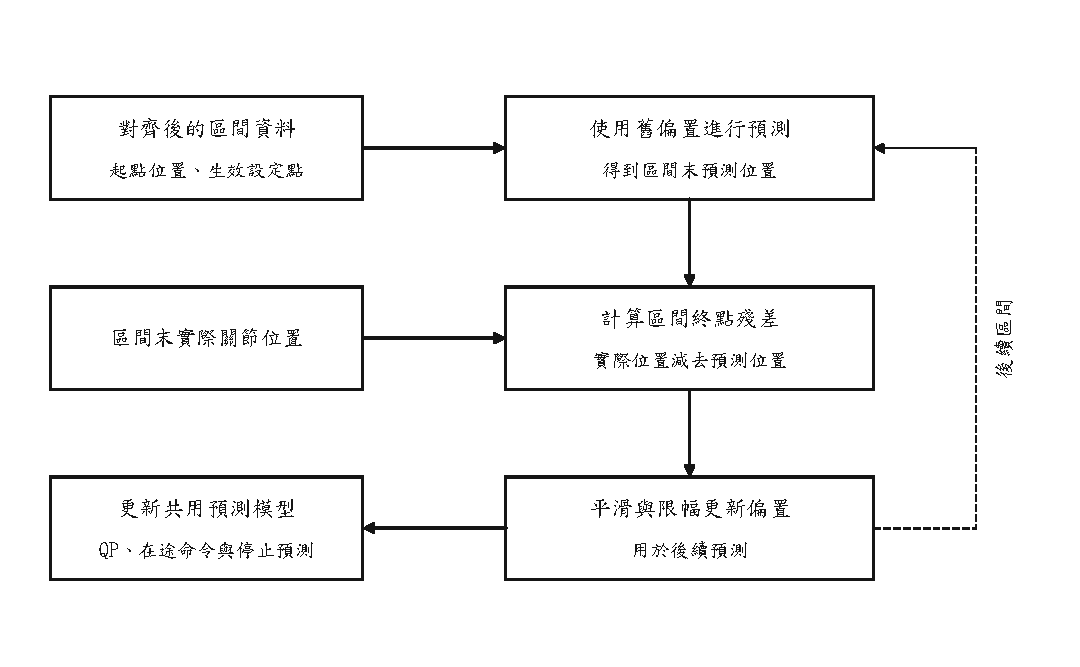
\includegraphics[width=0.98\textwidth]{figsrc/ch03/model_bias_estimation.pdf}
    \caption{模型偏置估測之區間殘差與共用模型更新}
    \label{fig:ch3_model_bias_estimation}
\end{figure}


% ==================================================
% 3.7.2 末端原始幾何目標與有界命令目標補償
% 位置：3.7.2 有界 TCP 目標補償公式與說明之後
% ==================================================
末端目標修正的作用如\cref{fig:ch3_tcp_target_compensation}所示。圖中以單一位置分量說明原始幾何目標、實際末端位置及補償後命令目標的差異；補償量只改變控制器追蹤的命令目標，完成條件仍以原始幾何目標判定。

\begin{figure}[htbp]
    \centering
    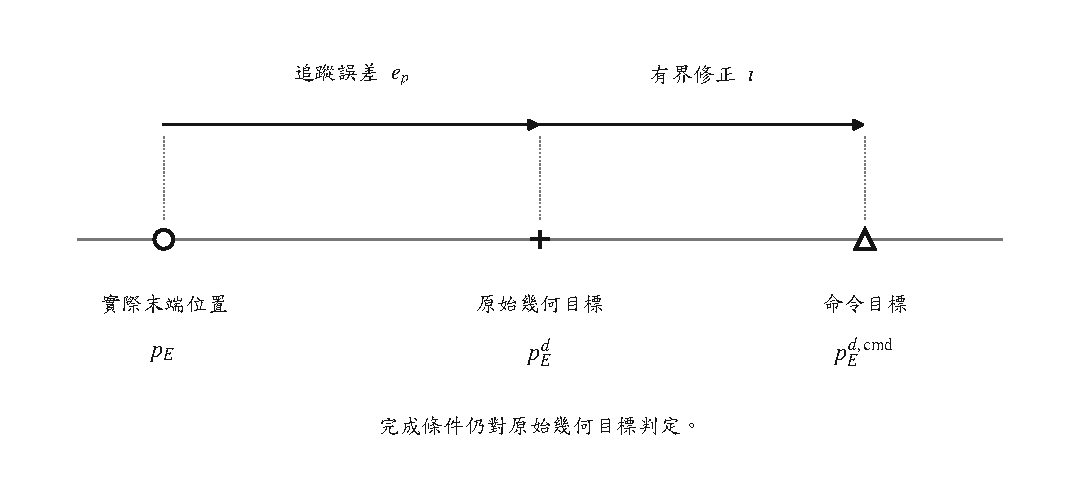
\includegraphics[width=0.98\textwidth]{figsrc/ch03/tcp_target_compensation.pdf}
    \caption{末端原始幾何目標與有界命令目標補償}
    \label{fig:ch3_tcp_target_compensation}
\end{figure}

